\begin{center}
\begin{tabular}{@{}ccc@{}}
\begin{tikzpicture}[x=.5pt,y=-.5pt,line width=.65pt,line cap=round,line join=round,font=\scriptsize]
\useasboundingbox (125,240) rectangle (335,590);
\draw (269,253) .. controls (289,250) and (298,276) .. (301,315)
 .. controls (309,388) and (306,464) .. (276,470)
 .. controls (244,480) and (237,422) .. (236,366)
 .. controls (233,313) and (238,252) .. (269,253);
\fill (270,361) circle[radius=1.1pt];
\node at (270,349) {0};\node at (222,349) {2};\node at (315,349) {2};
\node at (180,518) {[Bahn]};\node at (270,518) {I};
\node at (270,570) {\(\mathrm{E}\leqq0.36\)};
\end{tikzpicture}
&
\begin{tikzpicture}[x=.5pt,y=-.5pt,line width=.65pt,line cap=round,line join=round,font=\scriptsize]
\useasboundingbox (390,240) rectangle (580,590);
\draw (466,253) .. controls (481,255) and (498,255) .. (510,253);
\draw (466,253) .. controls (504,283) and (520,326) .. (519,364)
 .. controls (518,411) and (491,449) .. (464,470);
\draw (510,253) .. controls (475,281) and (457,324) .. (457,362)
 .. controls (455,408) and (481,447) .. (508,470);
\draw (464,470) .. controls (480,468) and (494,468) .. (508,470);
\fill (488,359) circle[radius=1.1pt];
\node at (488,348) {0};\node at (534,348) {2};\node at (488,263) {4};
\node at (488,518) {II};
\end{tikzpicture}
&
\begin{tikzpicture}[x=.5pt,y=-.5pt,line width=.65pt,line cap=round,line join=round,font=\scriptsize]
\useasboundingbox (610,240) rectangle (800,590);
\draw (657,255) .. controls (688,265) and (722,267) .. (750,257);
\draw (657,255) .. controls (689,283) and (712,325) .. (713,363)
 .. controls (715,406) and (692,445) .. (660,472);
\draw (750,257) .. controls (719,283) and (696,324) .. (696,363)
 .. controls (694,409) and (720,452) .. (752,476);
\draw (660,472) .. controls (692,464) and (725,464) .. (752,476);
\fill (704,366) circle[radius=1.1pt];
\node at (704,353) {0};\node at (727,353) {2};\node at (704,284) {4};
\node at (704,520) {III};
\end{tikzpicture}
\\[9pt]
\begin{tikzpicture}[x=.5pt,y=-.5pt,line width=.65pt,line cap=round,line join=round,font=\scriptsize]
\useasboundingbox (830,240) rectangle (1020,590);
\draw (870,263) .. controls (902,275) and (946,278) .. (975,265);
\draw (870,263) .. controls (901,289) and (922,329) .. (923,352)
 -- (923,382) .. controls (921,423) and (898,458) .. (871,478);
\draw (975,265) .. controls (945,290) and (925,330) .. (923,352)
 -- (923,382) .. controls (925,424) and (949,460) .. (979,480);
\draw (871,478) .. controls (906,465) and (946,468) .. (979,480);
\node at (923,299) {4};\node at (947,357) {2};
\node at (923,526) {IV};\node at (928,575) {\(\mathrm{E}=0.6\)};
\end{tikzpicture}
&
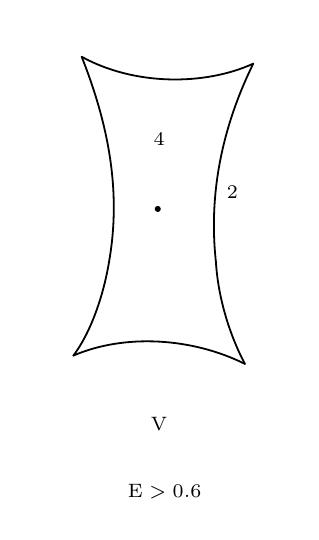
\begin{tikzpicture}[x=.5pt,y=-.5pt,line width=.65pt,line cap=round,line join=round,font=\scriptsize]
\useasboundingbox (1040,240) rectangle (1230,590);
\draw (1079,261) .. controls (1117,282) and (1168,282) .. (1203,266);
\draw (1079,261) .. controls (1100,314) and (1107,361) .. (1099,408)
 .. controls (1094,439) and (1083,464) .. (1073,477);
\draw (1203,266) .. controls (1179,315) and (1171,363) .. (1176,409)
 .. controls (1178,442) and (1190,470) .. (1197,483);
\draw (1073,477) .. controls (1110,461) and (1159,464) .. (1197,483);
\fill (1134,371) circle[radius=1.1pt];
\node at (1135,321) {4};\node at (1188,359) {2};
\node at (1135,526) {V};\node at (1139,575) {\(\mathrm{E}>0.6\)};
\end{tikzpicture}
&
\end{tabular}
\end{center}
